\pgfdeclarelayer{background}
\pgfdeclarelayer{foreground}
\pgfdeclarelayer{m-f}
\pgfdeclarelayer{main}

\pgfsetlayers{background,foreground}
\colorlet{LightBlue}{blue!10!white}
\colorlet{DarkBlue}{blue!80!white}

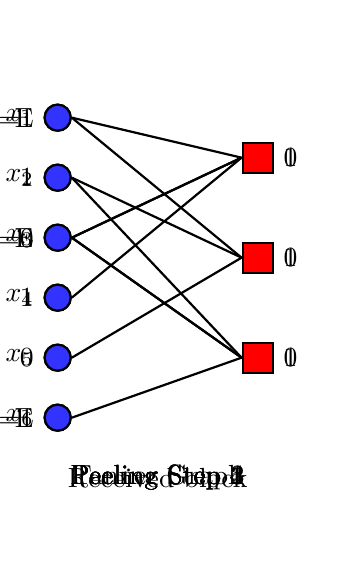
\begin{tikzpicture}[scale=1.0]
\clip (-0.15in,0.15in) rectangle (1.3in,-2.5in);

\def\n     {6}   % #-Variable nodes
\def\m     {3}  % #-Check nodes
\def\nodewidth{0.15in}
\def\nodegapVN{0.3in}
\def\nodegapCN{0.5in}

\tikzstyle{check} = [rectangle, draw, text centered, thick, fill=red,
                          minimum height=\nodewidth, minimum width=\nodewidth]
\tikzstyle{bit} = [circle, draw, text centered, thick, fill=LightBlue,
                          radius=0.5*\nodewidth]
\tikzstyle{bitpeeled} = [circle, draw, text centered, thick, fill=DarkBlue,
                          radius=0.5*\nodewidth]

\begin{pgfonlayer}{background}
%\draw[gray,step=0.5in] (-0.15in,0.15in) grid (1.5in,-2.5in);
\foreach \vn in {1,...,\n}{
  \node[bit] (vn\vn) at (0,-\vn*\nodegapVN) {};
 }

 \foreach \cn in {1,...,\m}{
  \node[check] (cn\cn) at (1in,-\cn*\nodegapCN) {};
 }
\end{pgfonlayer}



\begin{pgfonlayer}{foreground}

%Text to left of VN
\visible<1>{
\foreach \vn in {1,...,\n}{
  \node[left] (nodetxt) at (vn\vn.west) {\normalsize{$x_\vn$}};
 	}  	
}

\visible<2-8>{
\foreach \vn/\txt in {2/1,4/1,5/0}{
\node[left] (nodetxt) at (vn\vn.west) {\normalsize{\txt}};
 	}	
}

\visible<2-3>\node[left] (nodetxt) at (vn1.west) {\normalsize{E}};
\visible<2-5>\node[left] (nodetxt) at (vn3.west) {\normalsize{E}};
\visible<2-7>\node[left] (nodetxt) at (vn6.west) {\normalsize{E}};


\visible<4-8>\node[left] (nodetxt) at (vn1.west) {\normalsize{E=1}};
\visible<6-8>\node[left] (nodetxt) at (vn3.west) {\normalsize{E=0}};
\visible<8>\node[left] (nodetxt) at (vn6.west) {\normalsize{E=1}};

%Edges
\uncover<1-2>{
\foreach \vn/\cn in {2/2,2/3,4/1,5/2}{
 \draw[thick] (vn\vn.east)--(cn\cn.west);
  }
}

\visible<1-3>\draw[thick] (vn1.east)--(cn2.west);
\visible<1-4>\draw[thick] (vn1.east)--(cn1.west);

\visible<1-5>\draw[thick] (vn3.east)--(cn1.west);
\visible<1-6>\draw[thick] (vn3.east)--(cn3.west);

\visible<1-5>\draw[thick] (vn3.east)--(cn1.west);
\visible<1-6>\draw[thick] (vn3.east)--(cn3.west);

\visible<1-7> \draw[thick] (vn6.east)--(cn3.west);

%% Peeled bits color
\uncover<3-8>{
  \foreach \vn in {2,4,5}{
    \node[bitpeeled] () at (vn\vn) {};
    }
  }
 \visible<4-8>\node[bitpeeled] () at (vn1) {};
 \visible<6-8>\node[bitpeeled] () at (vn3) {};
  \visible<8>\node[bitpeeled] () at (vn6) {};

%Check node values
\visible<2,5,6,7,8> \node[right] (nodetxt) at (cn1.east) {\normalsize{0}};
\visible<3,4> \node[right] (nodetxt) at (cn1.east) {\normalsize{1}};

\visible<2,4,5,6,7,8> \node[right] (nodetxt) at (cn2.east) {\normalsize{0}};
\visible<3> \node[right] (nodetxt) at (cn2.east) {\normalsize{1}};

\visible<2,6,7,8> \node[right] (nodetxt) at (cn3.east) {\normalsize{0}};
\visible<3,4,5> \node[right] (nodetxt) at (cn3.east) {\normalsize{1}};



%% Text at the bottom
\visible<1> \node[minimum width=10cm] (txt) at (0.5in,-7*\nodegapVN) {Tanner Graph};
\visible<2> \node[minimum width=10cm] (txt) at (0.5in,-7*\nodegapVN) {Received block};
\visible<3> \node[minimum width=10cm] (txt) at (0.5in,-7*\nodegapVN) {Peeling Step 1};
\visible<4-5> \node[minimum width=10cm] (txt) at (0.5in,-7*\nodegapVN) {Peeling Step 2};
\visible<6-7> \node[minimum width=10cm] (txt) at (0.5in,-7*\nodegapVN) {Peeling Step 3};
\visible<8> \node[minimum width=10cm] (txt) at (0.5in,-7*\nodegapVN) {Peeling Step 4};

\end{pgfonlayer}
\end{tikzpicture} 